% Sample Paper for Poster Conference
%( without guarantee:-)) 
%send your comment to xrund@fel.cvut.cz
%
\documentclass{poster15}
% 
%----------------------------------------------------------
%             THIS IS THE PLACE FOR YOUR FAVORITE PACKAGES
%
\usepackage[utf8]{inputenc}%
%\usepackage{babel}% 
%\usepackage{czech}%
%\usepackage{psfrag}
%\usepackage{amsmath}
%\usepackage{pifont,amssymb}
\usepackage{amssymb,amsmath}

\usepackage{url}
\usepackage{listings}

\lstset{basicstyle=\small\ttfamily}

\begin{document}
%----------------------------------------------------------

%----------------------------------------------------------
%               THIS IS THE PLACE OF THE TITLE
%
\title{YodaQA: A Modular Question Answering System Pipeline}
%----------------------------------------------------------
%               THIS IS THE PLACE FOR THE AUTHORS NAMES AND THE TITLE FOR HEADINGS
%
\headtitle{P. BAUDIŠ, YodaQA Question Answering}
%----------------------------------------------------------
%               THIS IS THE PLACE FOR THE AUTHORS NAMES - ALL AUTHORS MUST HAVE A STUDENT STATUS!!!

%
\author{Petr Baudiš}
%----------------------------------------------------------
%              THIS IS THE PLACE FOR AFFILIATIONS
%
\affiliation{%
	Dept.\ of Cybernetics, Czech Technical University, Technická 2, 166 27 Praha, Czech Republic
}
  \email{baudipet@fel.cvut.cz}
%--------------------------------------------------------------


\maketitle

%----------------------------------------------------------
%               THIS IS THE PLACE FOR ABSTRACT

\begin{abstract}
	Question Answering as a sub-field of information retrieval
	and information extraction is recently enjoying renewed
	popularity, triggered by the publicized success of IBM Watson in
	the Jeopardy! competition.  But Question Answering research is
	now proceeding in several semi-independent tiers depending on the
	precise task formulation and constraints on the knowledge base,
	and new researchers entering the field can focus only on
	various restricted sub-tasks as no modern full-scale software
	system for QA has been openly available for research so far.

	By our YodaQA system that we introduce here,
	we seek to reunite and boost research efforts
	in Question Answering, providing a modular, open source
	pipeline for this task --- allowing integration of
	various knowledge base paradigms,
	answer production and analysis strategies and using a machine
	learned models to rank the answers.  Within this pipeline,
	we also supply a baseline QA system inspired by DeepQA
	with solid performance
	and propose a reference experimental setup
	for easy future performance comparisons.

	In this paper, we review the available open QA platforms,
	present the architecture of our pipeline,
	the components of the baseline QA system, and also analyze
	the system performance on the reference dataset.
\end{abstract}


%----------------------------------------------------------
%               THIS IS THE PLACE FOR KEYWORDS
\begin{keywords}
	Question answering, information retrieval, information extraction,
	linked data, natural language processing, Apache UIMA,
	software engineering.
\end{keywords}

%----------------------------------------------------------
%               HERE WRITE YOUR PAPER

\section{Introduction}

We consider the Question Answering problem --- a function of
unstructured user query that returns the information queried for.
This is a harder problem than a linked data graph search (which requires
a precisely structured user query) or a generic search engine (which
returns whole documents or sets of passages instead of the specific
information).
The Question Answering task is however a natural extension of a search
engine, as currently employed e.g.\ in Google Search \cite{googleKG}
or personal assistants like Apple Siri, and with the high
profile IBM Watson Jeopardy! matches \cite{WatsonOverview}
it has became a benchmark of progress in AI research.
As we are interested in a general purpose QA system, we will consider
an ``open domain'' general factoid question answering, rather than
domain-specific applications, though we keep flexibility in this direction
as one of our goals.

Diverse QA system architectures have been proposed in the last 15 years,
applying different approaches to information retrieval.  A full survey
is beyong the scope of this paper, but let us outline at least the most
basic choices we faced when designing our system.

Perhaps the most popular approach in QA research has been restricting
the task to querying structured knowledge bases, typically using the
RDF paradigm and accessible via SPARQL\@.  The QA problem can
be then rephrased as learning a function translating free-text user query
to a structured lambda expression or SPARQL query. \cite{Semantic2013Berant} \cite{Semantic2014Bordes}
We prefer to focus on unstructured datasets as the coverage of the system
as well as domain versatility increases dramatically; building a combined
portfolio of structured and unstructured knowledge bases
is then again an obvious extension.

When relying on unstructured knowledge bases, a common strategy is to offload
the information retrieval on an external high-quality web search engine
like Google or Bing (see e.g.\ the \textbf{Mulder} system \cite{MulderKwok}
or many others).
We make a point of relying purely on local information sources.
While the task becomes noticeably harder,
%as we index significantly less data and search results may not be that well sorted,
we believe the result is a more
universal system that could be readily refocused on a specific domain
or proprietary knowledge base, and also a system more appropriate as
a scientific platform as the results are fully reproducible over time.

Finally, a common restriction of the QA problem concerns only selecting
the most relevant answer-bearing passage, given a tuple of input question
and set of pre-selected candidate passages \cite{WangQAGrammar}.
This Answer Sentence Selection task is certainly
worthwhile as a component of a QA system but does not form a full-fledged
system by itself.
It may be argued that returning a whole passage is more useful for the user than a direct narrow answer,
but this precludes any reasoning or other indirect answer synthesis on the part of the system,
while the context and supporting evidence can be still provided by the user interface.
Direct answer output may be also used in a more general AI reasoning engine.

In this paper, we present our open source Question Answering system
\textbf{brmson YodaQA}.  This is not the only open source QA framework
currently available, but we found our goals not entirely compatible
with any of the other systems we investigated.
Specifically, we aim to build a system that
(A) provides an end-to-end, universal pipeline integrating different
knowledge base paradigms in a modular fashion;
(B) is domain flexible and could cater even to the long tail of rarer
question subjects, therefore has minimum of fixed categories and hand-coded rules.

In contrast, the classic QA system \textbf{OpenEphyra} \cite{Ephyra2006}
operates on the basis of fixed question categories with hand-crafted rules,
and puts emphasis on querying web search engines.
The \textbf{OAQA} initiative \cite{OAQATowards} has developed a basic QA framework,
but does not provide an end-to-end pipeline and its usage of UIMA has
in our opinion severe design limitations (see below).
The \textbf{WatsonSim} system \cite{WatsonSim} has begun developing independently
during the course of our own work and it works on Jeopardy! statements rather
than questions.

\textbf{Jacana} \cite{TreeEdit2013Yao} \cite{TreeEditIR2013Yao}
is a promising set of loosely coupled QA-related methods
and algorithms, focused on machine learning of textual entailment.  It is
not meant to be a full QA framework and using it as an end-to-end pipeline
is not straightforward, but integration of the Jacana implementation as
modules in YodaQA is our long-term plan.

\textbf{OpenQA} \cite{OpenQA} is a recently introduced end-to-end QA pipeline platform
also developed independently during the course of our work, and shares our
goal of a common research platform in the field.  However, the approach
is very different, as OpenQA is more of a portfolio-style engine with
mostly independent pipelines which have their candidate answers combined,
while YodaQA emphasizes modularity on the pipeline stage level,
with e.g.\ all answer producers sharing a common answer analysis stage.

The rest of the paper is structured as follows.  We outline the general structure
of our framework in Sec.~\ref{sec:yodaqaarch}.  We then
describe the current reference implementation of the pipeline components
in Sec.~\ref{sec:yodaqarefpip}.  We propose a common experimental setup
and analyze the system performance in Sec.~\ref{sec:results}.
We conclude with a summary of our contributions
and an outline of future extensions in Sec.~\ref{sec:conclusion}.

\begin{figure*}[ht]
\begin{center}
\resizebox{15cm}{!}{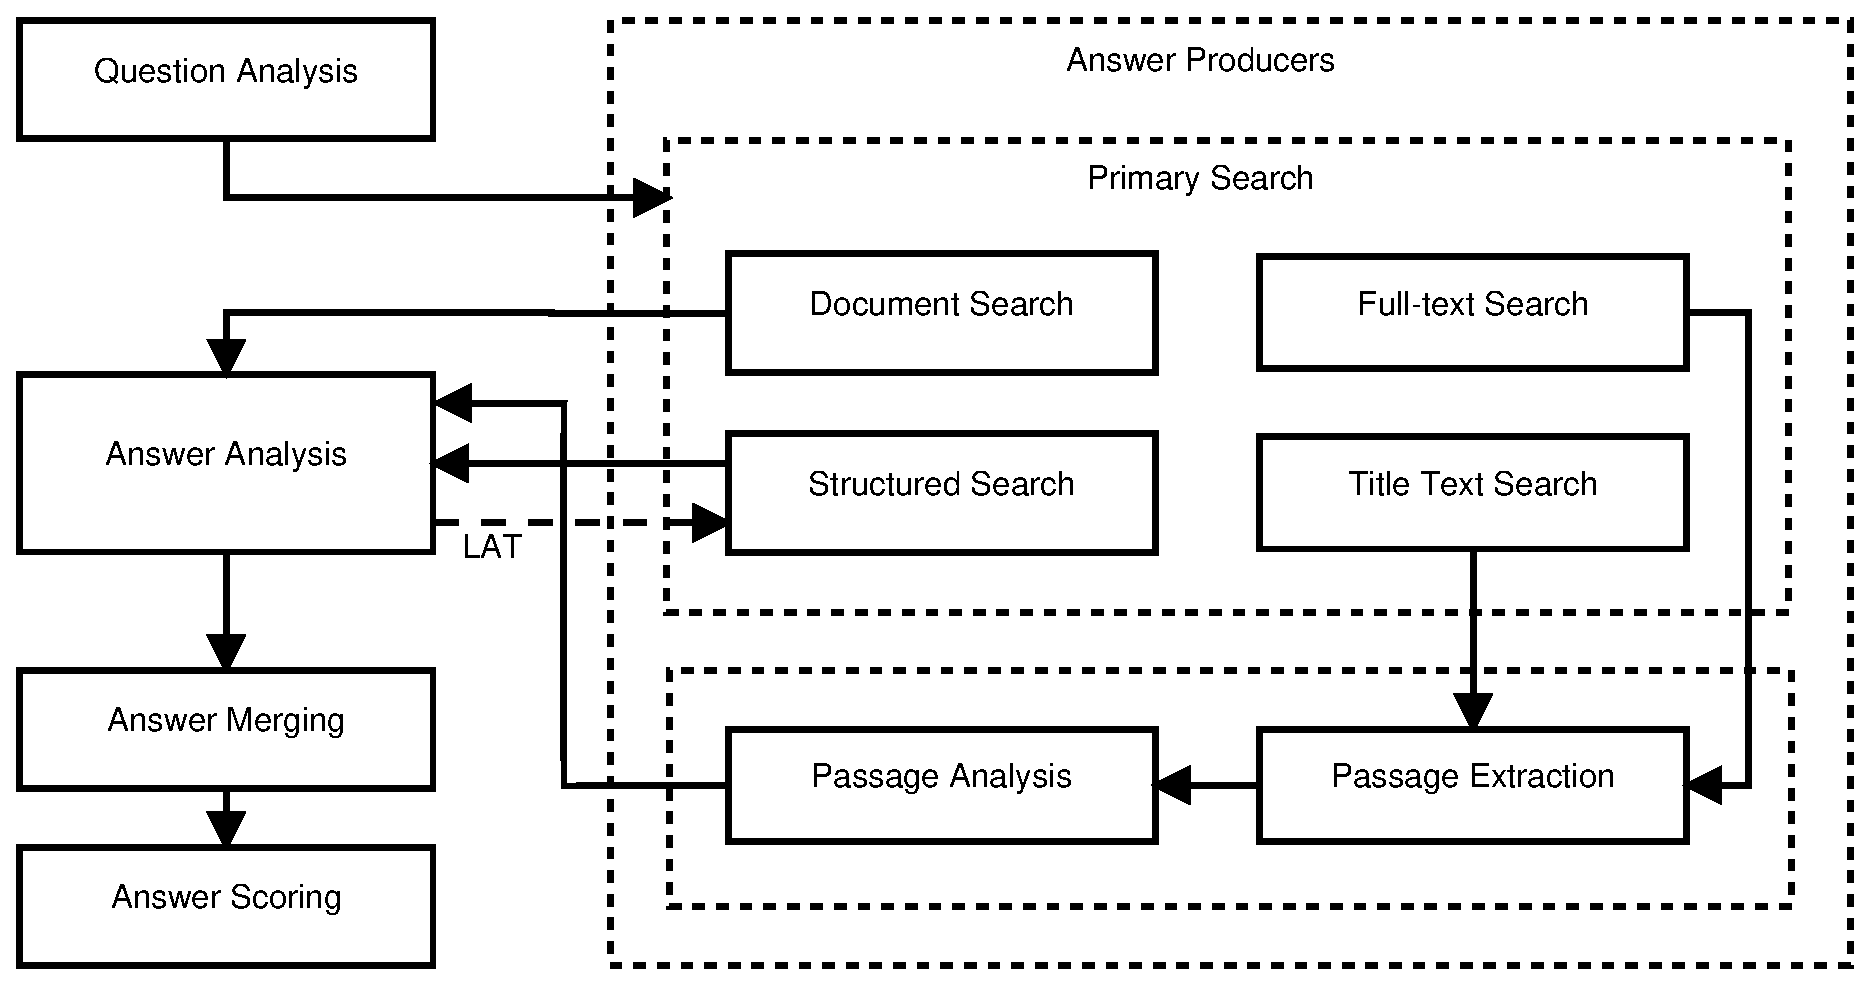
\includegraphics{yodaqa-arch.eps}}
%\vspace*{-0.75cm}
\captionwide{The general architecture of the YodaQA pipeline.  Present but unused final pipeline portions not shown.}
\label{fig:arch}
\end{center}
\end{figure*}%\vspace{5mm}


\section{YodaQA Pipeline Architecture}
\label{sec:yodaqaarch}

The goals for our system ``brmson YodaQA'' are to provide an open source
Question Answering platform that can serve both as scientific research
testbed and a practical system. The pipeline is implemented mainly in Java,
using the popular Apache UIMA framework \cite{UIMA}.  Extensive support
tooling is included within the package.

Unlike OAQA, in YodaQA each artifact (question, search result, passage,
candidate answer) is represented as a separate UIMA CAS, allowing easy
parallelization and easy leverage of pre-existing NLP UIMA components;
we also put emphasis on aggressive compartmentalization
of different tasks to interchangeable annotators rather than using
UIMA just for high level flow and annotation storage.

The framework is split in several Java packages: \textbf{io} takes care
of retrieving questions and returning answers, \textbf{pipeline} contains
classes of the general pipeline stages, \textbf{analysis} contains
modules for various analysis steps, \textbf{provider} has interfaces
to various external resources and \textbf{flow} carries UIMA helper classes.

The system maps an input question to ordered list of answer candidates in a pipeline fashion,
with the flow as in Fig.~\ref{fig:arch}, encompassing the following stages:

\begin{itemize}
\item \textbf{Question Analysis} extracts natural language features from the question text and produces QA features based on them (clues, type, etc.).
\item \textbf{Answer Production} generates candidate answers based on the question.
	Typically, this happens by performing a \textbf{Primary Search} in the knowledge bases according to the question clues,
	and either directly using search results as candidate answers
	or filtering relevant passages from these (the \textbf{Passage Extraction})
	and generating candidate answers from picked passages (the \textbf{Passage Analysis}).
\item \textbf{Answer Analysis} generates various answer features based on detailed analysis (most importantly, type determination and coercion to question type).
\item \textbf{Answer Merging and Scoring} consolidates the set of answers, removing duplicates and using a machine learned classifier to score answers by their features.
\item \textbf{Successive Refining} (optional) prunes the set of questions in multiple phases, interjecting some extra tasks (evidence diffusion and gathering additional evidence).
\end{itemize}

The basic pipeline flow is much inspired by the DeepQA model
of IBM Watson \cite{WatsonPipeline}.  Throughout the flow, answer features
are gradually accumulated and some results of early flow stages (especially
the question analysis) are carried through the rest of the flow.


\section{YodaQA Reference Pipeline}
\label{sec:yodaqarefpip}

The particular Question Answering problem considered in the reference
pipeline is finding a precise (narrowly phrased) answer to a naturally
phrased English question, based on both unstructured (English Wikipedia,
\textit{enwiki})
and structured (DBpedia \cite{dbpedia}, Freebase \cite{freebase}) knowledge bases.

In our pipeline, we build on existing third-party NLP analysis tools,
in particular Stanford CoreNLP (Segmenter, POS-Tagger, Parser) \cite{StanfordCoreNLP} \cite{StanfordNNParser},
OpenNLP (Segmenter, NER) \cite{OpenNLP} and LanguageTool (Segmenter, Lemmatizer).%
\footnote{\url{http://www.languagetool.org/}}%
\footnote{Sometimes, different pipeline components default to different
NLP backends to perform the same task, e.g.\ segmentation,
based on empirically determined best fit.}
NLP analysis backends are freely interchangeable thanks
to the DKPro UIMA interface \cite{DKPro}.
For semantic analysis, we also rely heavily on the WordNet lexicon \cite{WordNet}.

For a practical illustration of the pipeline processing two particular example questions,
please follow Fig.~\ref{fig:exEnder} and~\ref{fig:exIditarod}.


\subsection{Question Analysis}

During question analysis,
produce a part-of-speech tagging and dependency parse of the question text,
recognize named entities and,
roughly inspired by the DeepQA system \cite{WatsonQuestion},
heuristically generate several QA features: Clues, Focus, and LAT.

\textbf{Clues} represent keywords in the question that determine its content
and are used to query for candidate answers.
Clues based on different question components are assigned different weight
(used in search retrieval and passage extraction, determined empirically) ---
in ascending other, all noun phrases, noun tokens and the selection verb (SV);
the LAT (see below);
named entities;
the question sentence subject (determined by dependency parse).
If the clue text corresponds to an \textit{enwiki} article name or redirect alias,
its weight is boosted and it is flagged as a \textbf{concept clue}.

\textbf{Focus} is the center point of the question sentence
indicating the queried object.
Six simple hand-crafted heuristics extract the focus based on the dependency parse.
``name of ---'' constructions are traversed.

\textbf{LAT} (Lexical Answer Type) describes a type of the answer that would fit the question.
This type is not of a pre-defined category but may be an arbitrary English noun,
like in the DeepQA system. \cite{WatsonTyCor}
The LAT is derived from the focus, except question words are mapped to nouns
(``where'' to ``location'', etc.)
and adverbs (like ``hot'') are nominalized (to ``temperature'') using WordNet relations.

\subsection{Unstructured Answer Sources}

The primary source of answers in our QA system is keyword search in free-text knowledge base,
in our default setting the \textit{enwiki}.
While the information has no formal structure, we take advantage of the organization of the \textit{enwiki} corpus
where entity descriptions are stored in articles that bear the entity name as title
and the first sentence is typically an informative short description of the entity.
Our search strategies are analogous to basic DeepQA free-text information retrieval methods \cite{WatsonIR}.
We use the Apache Solr\footnote{\url{http://lucene.apache.org/solr/}} search engine (frontend to Apache Lucene).

\textbf{Title-in-clue search} \cite{WatsonIR} looks for the question clues in the article titles,
essentially aiming to find articles that describe the concepts touched in the question.
The first sentence of the top six articles (which we assume is its summary)
is then used in passage analysis (see below).

\textbf{Full-text search} \cite{WatsonIR} runs a full-text clue search in the article texts and titles,
considering the top six results.
The document texts are split to sentences which are treated as separate passages
and scored based on sum of weights of clues occuring in each passage\footnote{%
The \textit{about-clues} which occur in the document title have their weight divided by four (as determined empirically).}%
\footnote{We also carry an infrastructure for machine learning models scoring candidate passages,
		but they have not been improving performance so far.};
the top three passages from each document are picked for passage analysis.

\textbf{Document search} \cite{WatsonIR} runs a full-text clue search in the article texts;
top 20 article hits are then taken as potential responses,
represented as candidate answers by their titles.

\textbf{Concept search} retrieves articles whose titles (or redirect aliases) exactly match a question clue.
The first sentence and also passages extracted as in the full-text search are used for passage analysis.

Given a picked passage, the \textbf{passage analysis} process executes an NLP pipeline and generates candidate answers;
currently, the answer extraction strategy entails simply converting all named entities and noun phrases to candidate answers.
Also, object constituents in sentences where subject is the question LAT are converted to candidate answers.

\subsection{Structured Answer Sources}

Aside of full-text search, we also employ structured knowledge bases organized in RDF triples;
for each concept clue, we query for predicates with this clue as a subject
and generate candidate answers for each object in such a triple, with the predicate label seeded as one LAT of the answer.

In particular, we query the DBpedia \texttt{ontology} (curated) and \texttt{property} (raw infobox)
namespaces and the Freebase RDF dump.
For performance reasons, we limit the number of queried Freebase topics to 5 and retrieve only 40 properties per each;
due to this limitation, we have manually compiled a blacklist of skipped
``spammy'' properties based on past system behavior analysis
(e.g.\ location's \textit{people\_born\_here} or music artist's \textit{track}).

\subsection{Answer Analysis}

In the answer analysis, the system takes a closer look at the answer snippet
and generates numerous features for each answer.
The dominant task here is type coercion,
i.e.\ checking whether the answer type matches the question LAT.

The answer LAT is produced by multiple strategies:
\begin{itemize}
	\item Answers generated by a named entity recognizer have LAT corresponding to the triggering model;
		we use stock OpenNLP NER models \textit{date}, \textit{location}, \textit{money}, \textit{organization}, \textit{percentage}, \textit{person} and \textit{time}.
	\item Answers containing a number have a generic \textit{quantity} LAT generated.
	\item Answer focuses (the parse tree roots) are looked up in WordNet and \textit{instance-of} pairs are used to generate LATs (e.g.\ \textit{Einstein} is \textit{instance-of} \textit{scientist}).
	\item Answer focuses are looked up in DBpedia and its ontology is used to generate LATs.
	\item Answers originating from a structured knowledge base carry the property name as an LAT.
\end{itemize}

Type coercion between question and answer LATs is performed using the WordNet
hypernymy relation --- i.e.\ \textit{scientist} may be generalized to \textit{person}, or \textit{length} to \textit{quantity}.
We term the type coercion score \textbf{WordNet specificity} and exponentially decrease it
with the number of hypernymy traversals required.
Answer LATs coming from named entity recognizer and quantity are not generalized.
We never generalize further once within the \texttt{noun.Tops} WordNet domain and
based on past behavior analysis, we have manually compiled a further blacklist
of WordNet synsets that are never accepted as coercing generalizations
(e.g. \textit{trait} or \textit{social group}).

The generated features describe the origin of the answer (data source, search result score, clues of which type matched in the passage, distance-based score of adjacent clue occurences, etc.), syntactic overlaps with question clues and type coercion scores (what kind of LATs have been generated, if any type coercion succeeded, what is the WordNet specificity and whether either LAT had to be generalized).

\subsection{Answer Merge-and-Score}

The merging and scoring process also basically follows a simplified DeepQA approach \cite{WatsonScoring}.
Candidate answers of the same text (up to basic normalization, like \textit{the-} removal) are merged;
element-wise maximum is taken as the resulting answer feature vector
(except for the \texttt{\#occurences} feature, where a sum is taken).
To reduce overfitting, too rare features are excluded
(when they occur in less than $1\%$ questions and $0.1\%$ answers).

Supplementary features are produced for each logical feature --- aside of the original value,
a binary feature denoting whether a feature has \textit{not} been generated
and a value normalized over the full set of answers
so that the distribution of the feature values over the answer
has mean 0 and standard deviation 1.
The extended feature vectors are converted to a score $s \in [0,1]$
using a logistic regression classifier.
The weight vector is trained on the gold standard of a training dataset,
employing L2 regularization objective.  To strike a good precision-recall
balance, positive answers (which are about $p=0.03$ portion of the total)
are weighed by $0.5/p$.

\subsection{Successive Refining}

The pipeline contains support for additional refining and scoring phases.
By default, after initial answer scoring,
only the top 25 answers are kept with the intent of reducing noise for the next answer scoring classifier.
Answers are compared and those overlapping syntactically (prefix, suffix, or substring aligned with sub-phrase boundaries)
are subject to evidence diffusion where their scores are used as features of the overlapping answers.
Another answer scoring would be then performed, and the answer with the highest score is then finally output by the system.%
\footnote{There is also experimental support for additional evidence gathering phase, where the top 5 answers are looked up using the full-text search together with the question clues, and the number and score of hits are used as additional answer features and final answer rescoring is performed.  Nevertheless, we have not found this approach effective.}

However, while we have found these extra scoring steps beneficial with
weaker pipelines (in particular without the clue overlap features),
in the final pipeline configuration the re-scoring triggers significant
overfitting on the training set and we therefore ignore
the successive refining stage in the benchmarked pipeline.


\section{Performance Analysis}
\label{sec:results}

As we present performance analysis of our system,
we shall first detail our experimental setup;
this also includes discussion of our question dataset.

Then, we proceed with the actual results --- we measure the \textit{recall}
of the system (whether a correct answer has been generated and considered,
without regard to its score) and \textit{accuracy-at-one} (whether the
correct answer has been returned as the top answer by the system).
We find this preferrable to typical information retrieval measures like MRR or MAP
since in many applications, eventually only the single top answer output by the system
matters; however, we also show the \textit{mean reciprocial rank}
for each configuration and discuss the rank distribution of correct answers.

Aside of the performance of the default configuration, we also discuss
scaling of the system (extending the alotted answer time) and performance
impact of its various components (hold-out testing).

\subsection{Experimental Setup}

Our code is version tracked in a public GitHub repository
\url{https://github.com/brmson/yodaqa}, and the experiments presented
here are based on commit \texttt{f6c0cf6} (tagged as \texttt{v1.0}).
The quality of full-text search is co-determined by Solr version
(we use 4.6.0) and models of the various NLP components which are brought
in by DKPro version 1.7.0.
As for the knowledge bases, we use enwiki-20150112, DBpedia 2014,
Freebase RDF dump from Jan 11 2015, and WordNet 3.1.
Detailed instructions on setting up the same state locally (including
download of the particular dump versions and configuration files) are
distributed along the source code.

As a benchmark of the system performance, we use a dataset of 430 training
and 430 testing open domain factoid questions.
(For system development, exclusively questions from the training set are used.)
This dataset is based on the public question answering benchmark from
the main tasks of the TREC 2001 and 2002 QA tracks
with regural expression answer patterns%
\footnote{\url{http://trec.nist.gov/data/qa/2001_qadata/main_task.html} and 2002 analogically.}
and extended by questions asked
to a YodaQA predecessor by internet users via an IRC interface.
This dataset was further manually reviewed by the author,
ambiguous or outdated questions were removed
and the regex patterns were updated based on current data.
We refer to the resulting 867 question dataset as \texttt{curated} and
randomly split it to the training and testing sets.\footnote{The remaining
7 questions are left unused for now.}

An automatic benchmark evaluation system is distributed as part of the
YodaQA software package.  The system evaluates the training and test questions
in parallel and re-trains the machine learning models before scoring the answers.
Therefore, in all the modified system versions considered below, a model trained
specifically for that version is used for scoring answers.

Our benchmark is influenced by two sources of noise.
First, the answer correctness is determined automatically by matching a predefined regex,
but this may yield both false positives and false negatives.%
\footnote{For example numerical quantities with varying formatting and units are notoriously tricky to match by a regular expression.}
Second, during training the models are randomly initialized and therefore their final
performance on a testing set flutters a little.

\subsection{Benchmark Results}

\begin{figure*}[t]
% increase table row spacing, adjust to taste
\renewcommand{\arraystretch}{1.3}
\centering
\begin{tabular}{|c|cccc|}
\hline
Pipeline & Recall & Accuracy-at-1 & MRR & time \\ \hline \hline
default & 79.3\% & 32.6\% & 0.420 & 28.8s \\
% test  1119b6c 2015-03-09 Merge branch 'master... 144/289/430 33.5%/67.2% avgscore 0.504 mrr 0.424 avgtime 283643.667	+uv +uv
% test u1119b6c 2015-03-09 Merge branch 'master... 140/341/430 32.6%/79.3% avgscore 0.602 mrr 0.420 avgtime 283440.296
% test v1119b6c 2015-03-09 Merge branch 'master... 138/290/430 32.1%/67.4% avgscore 0.503 mrr 0.417 avgtime 283569.631
\hline
full-text scaling ($6\to12$ fetched results) & 82.3\% & 34.0\% & 0.430 & 50.0s \\
% test  e8e2f7b 2015-03-21 SolrFullPrimarySearc... 133/295/430 30.9%/68.6% avgscore 0.512 mrr 0.418 avgtime 12260.108	uv+ uv+
% test ue8e2f7b 2015-03-21 SolrFullPrimarySearc... 146/354/430 34.0%/82.3% avgscore 0.630 mrr 0.430 avgtime 11980.825
% test ve8e2f7b 2015-03-21 SolrFullPrimarySearc... 135/297/430 31.4%/69.1% avgscore 0.519 mrr 0.425 avgtime 12168.474

passage scaling ($3\to6$ picked passages) & 81.2\% & 31.4\% & 0.415 & 43.5s \\
% test  e1b3c91 2015-03-21 PassFilter: NUM_PICK... 137/296/430 31.9%/68.8% avgscore 0.509 mrr 0.419 avgtime 10368.150	v+u
% test ue1b3c91 2015-03-21 PassFilter: NUM_PICK... 135/349/430 31.4%/81.2% avgscore 0.616 mrr 0.415 avgtime 10088.654
% test ve1b3c91 2015-03-21 PassFilter: NUM_PICK... 146/294/430 34.0%/68.4% avgscore 0.516 mrr 0.432 avgtime 10275.724

document search scaling ($20\to40$) & 80.0\% & 31.6\% & 0.418 & 34.9s \\
% test  d8debbd 2015-03-21 SolrDocPrimarySearch... 135/292/430 31.4%/67.9% avgscore 0.499 mrr 0.410 avgtime 10859.761	u+v u+v
% test ud8debbd 2015-03-21 SolrDocPrimarySearch... 136/344/430 31.6%/80.0% avgscore 0.604 mrr 0.418 avgtime 10649.831
% test vd8debbd 2015-03-21 SolrDocPrimarySearch... 134/291/430 31.2%/67.7% avgscore 0.501 mrr 0.410 avgtime 10787.752

freebase scaling ($5\to10$ topics, $40\to80$ properties) & 79.8\% & 31.6\% & 0.416 & 29.8s \\
% test  6475b89 2015-03-22 FreebaseOntology: TO... 136/290/430 31.6%/67.4% avgscore 0.499 mrr 0.412 avgtime 6985.841
% test u6475b89 2015-03-22 FreebaseOntology: TO... 136/343/430 31.6%/79.8% avgscore 0.603 mrr 0.416 avgtime 6782.731
% test v6475b89 2015-03-22 FreebaseOntology: TO... 140/290/430 32.6%/67.4% avgscore 0.504 mrr 0.418 avgtime 6913.904

\hline
full-text hold-out & 49.5\% & 20.9\% & 0.277 & 5.8s \\
% test  cb27e81 2015-03-20 Merge branch 'master... 80/188/430 18.6%/43.7% avgscore 0.307 mrr 0.252 avgtime 1675.430	uv+
% test ucb27e81 2015-03-20 Merge branch 'master... 90/213/430 20.9%/49.5% avgscore 0.358 mrr 0.277 avgtime 1464.086
% test vcb27e81 2015-03-20 Merge branch 'master... 86/189/430 20.0%/44.0% avgscore 0.315 mrr 0.263 avgtime 1580.048

structured hold-out & 73.5\% & 29.1\% & 0.376 & 23.8s \\
% test  0659767 2015-03-20 YodaQA: Experimental... 113/265/430 26.3%/61.6% avgscore 0.448 mrr 0.362 avgtime 5443.057	uv+	vu+
% test u0659767 2015-03-20 YodaQA: Experimental... 125/316/430 29.1%/73.5% avgscore 0.546 mrr 0.376 avgtime 5261.876
% test v0659767 2015-03-20 YodaQA: Experimental... 125/267/430 29.1%/62.1% avgscore 0.461 mrr 0.380 avgtime 5371.852

type coercion hold-out & 79.3\% & 22.1\% & 0.314 & 30.0s \\
% test  a458fbf 2015-03-20 AnswerAnalysis: Expe... 90/246/430 20.9%/57.2% avgscore 0.388 mrr 0.304 avgtime 7249.693	uv+
% test ua458fbf 2015-03-20 AnswerAnalysis: Expe... 95/341/430 22.1%/79.3% avgscore 0.520 mrr 0.314 avgtime 7042.305
% test va458fbf 2015-03-20 AnswerAnalysis: Expe... 91/246/430 21.2%/57.2% avgscore 0.395 mrr 0.310 avgtime 7177.386

concept clues hold-out & 67.9\% & 23.0\% & 0.314 & 25.6s \\
% test  fdf189d 2015-03-20 QuestionAnalysis: Ex... 100/248/430 23.3%/57.7% avgscore 0.399 mrr 0.319 avgtime 6356.564	v+u
% test ufdf189d 2015-03-20 QuestionAnalysis: Ex... 99/292/430 23.0%/67.9% avgscore 0.490 mrr 0.314 avgtime 6104.581
% test vfdf189d 2015-03-20 QuestionAnalysis: Ex... 100/247/430 23.3%/57.4% avgscore 0.403 mrr 0.322 avgtime 6258.929

%external-resource LATs hold-out & 79.3\% & 22.1\% & 0.314 & 20.1s \\
% test  fe1b2e8 2015-03-20 AnswerAnalysis: Expe... 87/245/430 20.2%/57.0% avgscore 0.383 mrr 0.298 avgtime 5058.735	uv+
% test ufe1b2e8 2015-03-20 AnswerAnalysis: Expe... 95/341/430 22.1%/79.3% avgscore 0.520 mrr 0.314 avgtime 4888.693
% test vfe1b2e8 2015-03-20 AnswerAnalysis: Expe... 87/245/430 20.2%/57.0% avgscore 0.387 mrr 0.301 avgtime 4993.441

%fuzzy merging and evidence diffusion hold-out % & ...
% test  acbd992 2015-03-20 YodaQA pipeline: Exp... 129/290/430 30.0%/67.4% avgscore 0.497 mrr 0.405 avgtime 7364.049	uv+
% test uacbd992 2015-03-20 YodaQA pipeline: Exp... 139/341/430 32.3%/79.3% avgscore 0.602 mrr 0.420 avgtime 7131.604
% test vacbd992 2015-03-20 YodaQA pipeline: Exp... 135/290/430 31.4%/67.4% avgscore 0.503 mrr 0.413 avgtime 7276.565

clue overlap test hold-out & 79.3\% & 29.5\% & 0.390 & 30.1s \\
% test  65f5635 2015-03-20 AnswerAnalysis: Expe... 138/291/430 32.1%/67.7% avgscore 0.496 mrr 0.413 avgtime 7624.839	v+u
% test u65f5635 2015-03-20 AnswerAnalysis: Expe... 127/341/430 29.5%/79.3% avgscore 0.587 mrr 0.390 avgtime 7421.990
% test v65f5635 2015-03-20 AnswerAnalysis: Expe... 138/293/430 32.1%/68.1% avgscore 0.502 mrr 0.416 avgtime 7552.017
\hline
\end{tabular}
\vspace*{-0.2cm}
\captionwide{Benchmark results of various pipeline variants on the \textit{curated} test dataset.
MRR is the Mean Reciprocal Rank $|Q|\cdot\sum_{q\in Q}{1/r_q}$, time is the average time spent answering one question.}
\label{fig:bench}
\end{figure*}

\begin{figure}[t]
\begin{center}
\resizebox{85mm}{!}{\includegraphics{ranks.eps}}
\vspace*{-0.75cm}
\caption{Number of questions $x$ that output the correct answer ranked at least $y$.}
\label{fig:ranks}
\end{center}
\end{figure}%\vspace{5mm}

Benchmark results over various pipeline configurations are laid out in Fig.~2. %\ref{fig:bench}.
Aside of the general performance of the system,
it is instructive to look at the histogram of answer ranks
for the default pipeline, shown in Fig.~\ref{fig:ranks}.
We can observe that while accuracy-at-one is 32.6\%,
accuracy-at-five is already at 52.7\% of test questions.

The information retrieval parameters of the default pipeline are selected so
that answering a question takes about 30s on average on a single core of
AMD FX-8350 with 24GB RAM and SSD backed databases.
(Note that no computation pre-processing was done on the knowledge bases or datasets;
bulk of the time per question is therefore spent querying the search engine and parsing sentences,
making it an accurate representation of time spent on previously unseen questions.)
By raising the limiting
parameters, we can observe further recall increase, and in case of considering
more full-text search results, also a solid accuracy improvement.  Our system
could therefore meaningfully make use of further computing resources.

We also benchmarked performance with various components of the pipeline
disabled.  We can see that the full-text and structured knowledge bases
are complementary to a degree, but the full-text base is eventually
a much stronger answer source for our system.  Type coercion and detection
of the concept clues in the question are both important heuristics for
our QA system.

Comparison of performance across multiple systems is currently non-trivial,
unfortunately, as there is no universally agreed experimental setup so far
and not even published results on the TREC datasets
from the years we use are readily available.
OpenEphyra seemed to typically achieve accuracy-at-one of ``above 25\%'' on
the TREC datasets including our years according to \cite{Ephyra2006}.
In the Answer Sentence Selection task \cite{WangQAGrammar},
Jacana and similar textual entaliement systems are reported%
\footnote{See the \textbf{ACL Wiki} topic \textit{Question Answering (State of the art)}.}
to achieve MRR around 0.750 but this task represents
a significant restriction upon the general end-to-end QA pipeline.


\section{Conclusion}
\label{sec:conclusion}

We have described a modular question answering system which can be used
for effective mixing of both structured and unstructured knowledge bases,
is domain-flexible and highly amenable to further extensions in various
stages of its pipeline.  We put emphasis on universal, machine learned
methods and employ only a very limited amount of hand-crafted heuristics.

Meanwhile, the system is already demonstrating a reasonable open domain
factoid question answering performance, being able to answer a third
of the testing set questions correctly, over half of the questions
in top five answers, and considering
the correct answer for just about 80\% of the questions;
we have also shown a head-room for further
performance scaling by extending the available computational resources.

Our system is made available as open source under the highly permissive
Apache Software Licence%
\footnote{The GPL licence applies in case Stanford CoreNLP components are employed.}
and available for research collaboration on the GitHub social software hosting site.
We hope for our system to become an universal research platform for testing
of various question answering related strategies not only in isolation but also
measuring their effect in a real-world high performance end-to-end pipeline.
We also hope our work helps to clarify which of the numerous DeepQA
contributions are most essential to a minimal working modern QA system.


\subsection{Future Work}

We present here just the first version of a system that could be improved in
many desirable ways.  The software platform itself would benefit in particular
from a multi-threaded pipeline flow driver, a sophisticated user interface showing
the generated answer in context and hypertext, and sped up benchmarking
by caching information retrieval results (parsed picked passages) across runs.

Regarding algorithmic improvements, the most obvious candidates seem
a more sophisticated answer extraction strategy
(e.g.\ employing methods introduced in Jacana seems as a natural fit)
and more reliable type coercion as a negative evidence source;
we also hope that distributed representations might improve both areas.
We feel that without further large effort in feature engineering, logistic
regression is inadequate for scoring answers and we are seeing promising
preliminary results from employing random forests instead.

Analysis and model training would be improved with larger benchmark datasets
with more sophisticated correct answer verification.  Some sub-tasks
like type coercion would benefit from specialized datasets,
and passage extraction scoring could be tuned on the Answer Sentence Selection
dataset.

A robust heuristic for additional evidencing of most promising answers
remains as an open problem in our system.
While the natural idea of additional fulltext search combining the question and answer
has been beneficial with a less sophisticated pipeline, it does not improve performance
with our current featureful pipeline.


%----------------------------------------------------------
%               HERE IS EXAMPLE OF A FIGURE	
%		environment {figure} for one-column figure, {figure*} for two-column figure 
%	 	\caption{} for one-column caption, \captionwide{} for two-column figure
%
%\begin{figure}[ht!]
%\begin{center}
%\resizebox{65mm}{!}{\includegraphics{obr1.eps}}
%%\input{obr/dr1a.pstex_t}
%\caption{The description of a figure is of the same style as the description of a table; the figure itself is of the environment \texttt{figure}.
%} 
%\label{fig1}
%\end{center}
%\end{figure}%\vspace{5mm}
%
%		example of twocolumn figure - pay attention to figure numbering, may be wrong.
%
%\begin{figure*}[ht!]
%\begin{center}
%\resizebox{65mm}{!}{\includegraphics{obr1.eps}}
%\captionwide{The example of two-column figure and caption.
%} 
%\label{figwide}
%\end{center}
%\end{figure*}
%

%----------------------------------------------------------
%               THIS IS THE PLACE FOR  ACKNOWLEDGEMENTS
\section*{Acknowledgements}
This work was supported by the Grant Agency of the Czech Technical
University in Prague, grant No. SGS14/\allowbreak{}194/\allowbreak{}OHK3/\allowbreak{}3T/13.
The research was co-supervised by Dr.~Jan Šedivý and Dr. Petr Pošík.

%The authors are asked to pay special attention to the form of references. The NAMES OF AUTHORS should be typed in capitals, the \emph{Titles of Journals, Books or Proceedings} in italics with the first capital letter in all significant words. The tittles of articles are typed similarly as the basic text without the first capital letter in all words. Use the standart environment \verb+thebibliography+.

%----------------------------------------------------------
%               THIS IS THE PLACE FOR REFERENCES
%\begin{thebibliography}{9}
%\bibitem{paper}
%JAKUBOV\'A, I., RAIDA, Z. Exemplary Document for the paper in Radioengineering. \emph{Radioengineering}, 2006, vol. 15, no. 1, p. 1 - 2.
%\bibitem{book}
%AUTHOR, F., AUTHOR, S., AUTHOR, T. F. \emph{The Book}. 2nd ed. Humpolec: Nupish\&Publish, 1901.
%\bibitem{article}
%HUSN\'IK, L., LHOTSK\'A, L. About Poster 2005. In \emph{Proceedings of the 9th International Student Conference on Electrical Engineering POSTER 2005}. Prague (Czech Republic), 2005, p. 1 - 2.
%\end{thebibliography}

%\nocite{*}

\bibliographystyle{acm}
\bibliography{qa}


%----------------------------------------------------------
%               THIS IS THE PLACE FOR AUTHOR CV
\begin{authorcv}{Petr Baudiš}
	has received his Masters degree in
	Theoretical Computer Science at the Charles University in Prague.
	So~far, he has been working chiefly in the fields of Computer~Go
	and Continuous Black-box Optimization.
	Currently, he is a PhD student at the Czech Technical University
	%supervised by Dr. Petr Pošík and his
	and his interests are extending also to the topics related to
	information extraction from unstructured text corpora.
\end{authorcv}


\begin{figure}[t!]
% increase table row spacing, adjust to taste
\renewcommand{\arraystretch}{1.3}
\centering
\footnotesize
\begin{tabular}{|p{1.8cm}p{6cm}|}
\hline
Question Text & Who wrote Ender's Game? \\
Q. Analysis & \textbf{Focus:} who; \textbf{SV:} wrote; \textbf{LAT:} person \\
Question Clues & Ender's Game \textbf{(concept clue)}, wrote \\ \hline

Primary Search (DBpOnt.) & \textbf{author:} Orson Scott Card, \textbf{publisher:} Tor Books, \dots \\
Primary Search (DBpProp.) & (ibid), \textbf{cover artist:} John Harris, \textbf{Caption:} 2005, \dots \\
Primary Search (Freebase) & \textbf{Author} Orson Scott Card, \textbf{Characters} Valentine Wiggin, Hive Queen, \dots \\
Primary Search (concepts) & \textit{enwiki} Ender's Game \\
Primary Search (fulltext) %
	& \textbf{Query:} \texttt{+("wrote" OR titleText: "wrote")\^{}1.0 +("ender's Game" OR titleText:"ender's Game")\^{}1.1  ("wrote ender's Game "\textasciitilde4)\^{}2.1} \dots \\
	& \textbf{Found:} Ender's Game (series), Ender's Game, Ender's Game (film), Ender's Game (comics), Jane (Ender's Game), List of Ender's Game series planets \\
	& \textbf{Sample picked passages:} {\footnotesize Elaborating on characters and plot lines depicted in the novel, Card later wrote additional books to form the Ender's Game series.} \\
	& \dots {\footnotesize Valentine wrote an essay here comparing the priestly class to the skeletons of small vertebrates some time before Speaker for The Dead.} \\
Primary Search (titles) & Ender's Game, List of Ender's Game characters, Jane (Ender's Game), Ender's Game (short story), Ender's Game (film), Ender's Game (series) \\
	& \textbf{Sample first passage:} {\footnotesize "Ender's Game" is a 1985 military science fiction novel by American author Orson Scott Card.} \\
Primary Search (document) & Ender's Game (series), Elisabeth Hirsch, Orson Scott Card, Ender in Exile, Worthing Inn, Jane (Ender's Game), \dots \\ \hline

\textbf{Orscon Scott Card} & Structured primary search LAT \textit{author} (Wordnet hypernyms \textit{communicator}, \textit{person}, \textit{maker}, \textit{creator}); DBpedia LAT \textit{writer} (Wordnet hypernyms \textit{communicator}, \textit{person}); NER LAT \textit{person} \\
	& Successful type coercion match\textbf{!}, ``sharp'' (exact specific) match from NER LAT\textbf{!} \\
	& \textbf{occurences:} 19\textbf{!}, \textbf{origins:} document title, concept\textbf{!}, first passage, noun phrase, named entity, multiple origins, \textbf{other:} adjecent to a concept clue mention, no clue text overlap\textbf{!} \\
\textbf{Jane} & Structured primary search LAT \textit{character} (Wordnet hypernyms \textit{imaginary being}, \textit{creativity}, \textit{person}, \textit{message} and 36 others); NER LAT \textit{person} \\
	& Successful type coercion match\textbf{!}, ``sharp'' (exact specific) match from NER LAT\textbf{!} \\
	& \textbf{occurences:} 4, \textbf{origins} document title, first passage, noun phrase, named entity, multiple origins,
	\textbf{other:} no clue text overlap\textbf{!} \\ \hline

Final Answers & \textbf{Orson Scott Card} (0.99), Neal Shusterman (0.96), Elisabeth Hirsch (0.96), American author Orson Scott Card (0.96), \dots, List of Ender's Game series planets (0.94), Gavin Hood (0.94), Print (0.93), Jane (0.91), \dots \\ \hline
\end{tabular}
\vspace*{-0.2cm}
\caption{A sample of the pipeline process when (correctly) answering a training question. \textbf{!} indicates particularly distinguishing features.}
\label{fig:exEnder}
\end{figure}

\begin{figure}[t!]
% increase table row spacing, adjust to taste
\renewcommand{\arraystretch}{1.3}
\centering
\footnotesize
\begin{tabular}{|p{1.8cm}p{6cm}|}
\hline
Question Text & What is the name of the famous dogsledding race held each year in Alaska? \\
Q. Analysis & \textbf{Focus:} name; \textbf{SV:} held; \textbf{LAT:} race
	(by Wordnet hypernym: \textit{contest}, \textit{event}, \textit{biological group}, \textit{canal} and 9 others) \\
Question Clues & name, Alaska \textbf{(concept clues)}, race, held, famous, dogsledding, race, year \\ \hline

Primary Search (DBpOnt.) & \textbf{area Total:} 1717854.0, \textbf{country:} United States, \dots \\
Primary Search (DBpProp.) & (ibid), \textbf{West:} Chukotka, \textbf{Income Rank:} 4, \dots \\
Primary Search (Freebase) & \textbf{Date Founded} 1959-01-03, \textbf{Capital} Juneau, \dots \\
Primary Search (concepts) & \textit{enwiki} Alaska, Name \\
	& \textbf{Sample picked passages:} Various races are held around the state, but the best known is the Iditarod Trail Sled Dog Race, a 1150 mi trail from Anchorage to Nome (although the distance varies from year to year, the official distance is set at 1049 mi). \\
	& \dots Automobiles typically have a binomial name, a "make" (manufacturer) and a "model", in addition to a model year, such as a 2007 Chevrolet Corvette.\\
Primary Search (fulltext) & \textbf{Query:} \texttt{("the name of the famous dogsledding race held each year in Alaska" OR titleText:\dots)\^{}2.7 +("name" OR titleText:"name")\^{}2.6} \dots \\
	& \textbf{Found:} List of New Hampshire historical markers \\
Primary Search (titles) & Name of the Year, Danish Sports Name of the Year, List of organisms named after famous people, Alaska!, Alaska, Race of a Thousand Years \\
	& \textbf{Sample first passage:} The 2000 Race of a Thousand Years was an endurance race and the final round of the 2000 American Le Mans Series season. \\
Primary Search (document) & List of New Hampshire historical markers \\ \hline

\textbf{The 2000 Race of a Thousand Years} %
	& \textbf{Focus:} Race; DBpedia LAT \textit{automobile race}, \textit{auto race in australia}, \textit{new year celebration}, \textit{quantity} LAT \\
	& Successful type coercion match\textbf{!}, ``sharp'' (exact specific) match\textbf{!} \\
	& \textbf{occurences:} 1, \textbf{origins:}  first passage, noun phrase, \textbf{other:} adjecent to an LAT clue mention\textbf{!}, containing clue text \\
\textbf{Iditarod Trail Sled Dog Race} %
	& \textbf{Focus:} Race; DBpedia LAT \textit{sport}, \textit{sport in alaska}, \textit{alaska}, \textit{winter sport}, \textit{attraction}; (N.B. no \textit{race} LAT) \\
	& Successful type coercion match, loose match by generalization of \textit{attraction} to \textit{social event}\textbf{!} \\
	& \textbf{occurences:} 1, \textbf{origins}   passage by various clues, noun phrase,
	\textbf{other:} suffixed by clue text \\ \hline

Final Answers & The 2000 Race of a Thousand Years (0.97), --01-03 (0.94), List of New Hampshire historical markers (0.93), a binomial name, a "make" (manufacturer) and a "model", in addition to a model year, such as a 2007 Chevrolet Corvette (0.90), \textbf{the Iditarod Trail Sled Dog Race} (0.89), Various races (0.83), \dots \\ \hline
\end{tabular}
\vspace*{-0.2cm}
\caption{A sample of the pipeline process when (not quite correctly) answering a training question. \textbf{!} indicates particularly distinguishing features.}
\label{fig:exIditarod}
\end{figure}

\end{document}
